\documentclass{article}
\usepackage{graphicx}
\usepackage{amsmath}
\usepackage{amssymb}
\usepackage{natbib}
\renewcommand{\refname}{References}
\usepackage{url}

\title{A Differential Geometric Approach to Economic Forecast}

\author{Babak Emami}

\date{\today}

\begin{document}
\maketitle

\begin{abstract}


\end{abstract}

\section{Introduction}\label{section:introduction}

The usual approach to predicting price of an asset is to regress its
historical prices against a set of economic indicators. The problem
with this approach is that we still need knowledge of the future
values of these indicators. This is done by relying on estimate
forecasts of economic indicators which are often based on qualitative
methods, such as those in Blue Chip Economic Indicators and Blue Chip
Financial Forecasts~\cite{ref:blue-chip}. The forecasts in Blue Chip
publications are based on surveying top business economists in the
United States.

An approach is proposed to forecast economic variables without
depending on future values of any economic indicators. We look at the
economy as a multi-dimensional manifold~\cite{deFelice:1990}; each
dimension is an economic variable. These variables can be
macro-economic indicators or asset prices. We refer to this manifold
as an \textit{economic universe}. The observed values of economic
variables in a time period form a path in this universe. We refer to
this path as the \textit{economic path}. We then find a manifold for
which this path is a geodesic, governed by a system of ordinary
differential equations (ODEs). The future value of economic variables
can be predicted by solving this system of ODEs.

In what follows the mathematical framework used is discussed and a
methodology is proposed to infer the structure of economic universe
given a set of observed economic variables. Some results are presented
followed by a model parameter study. Finally, a trading algorithm is
proposed based on this approach.

\section{Mathematical Framework}\label{section:mathematical-framework}

Let us consider $n$ economic variables $x^{1}$ to $x^{n}$. The
realized values of these variables are smooth functions of time $t$;
$x^{i} = x^{i}(t)$. Moreover, let us consider a smooth real manifold
$M$ equipped with $(x^{1},x^{2},...,x^{n})$ as a coordinate
system. Each set of coordinate values $(x^{1},...,x^{n})$ denotes a
point $p$ on $M$. The realized values of these $n$ variables over a
period of time $[0,T]$ form a path over $M$, connecting $p_{0}$ =
$(x^{1}(0),...,x^{n}(0))$ to $p_{T}$ = $(x^{1}(T),...,x^{n}(T))$. This
path is smooth as $x^{i}$s are smooth functions of time. Now let us
add a constraint on $M$ by assuming that the above-mentioned path is a
geodesic of $M$. With this assumption, this path is governed by the
following system of ODEs,

\begin{equation}\label{eqn:geodesic}
\ddot{x}^{m} + \Gamma^{m}_{ab} \dot{x}^{a} \dot{x}^{b} = 0
\end{equation}

where $m,a,b \in [1,n] \cap \mathbb{N}$. The Christoffel symbols
$\Gamma^{m}_{ab}$ are in general functions of coordinates. Henceforth,
the summation convention is in effect unless stated otherwise.

We further assume manifold $M$ is equipped with a
Levi-Civita~\cite{deFelice:1990} connection and thus,

\begin{equation}\label{eqn:gamma}
\Gamma^{m}_{ab} = \frac{g^{ml}}{2} ( \frac{\partial g_{al}}{\partial
  x^{b}} + \frac{\partial g_{lb}}{\partial x^{a}} - \frac{\partial
  g_{ab}}{\partial x^{l}} )
\end{equation}

where $g_{ab}$ is the metric tensor (that is a symmetric,
non-degenerate, second order covariant tensor), and $g^{ab}$ is the
inverse of $g_{ab}$. Because the metric tensor is symmetric we have,

\begin{equation}\label{eqn:gamma-symmetry}
\Gamma^{m}_{ab} = \Gamma^{m}_{ba}
\end{equation}

In the current work, we assume that Christoffel symbols are
constant. This is a sufficient (but not necessary) condition for the
manifold to have a constant curvature. This assumption is rather
strong and as such we should revisit this subject in the near
future. We further assume that the metric tensor, $g_{ab}$ is
diagonal. Looking at Eq.~\ref{eqn:gamma}, this assumption indicates,

\begin{equation}\label{eqn:gamma-diagonal-metric}
\Gamma^{m}_{ab}|_{m \ne a \ne b} = 0
\end{equation}

To further simplify the problem, we assume that variables of interest
are in fact $y^{m} = \frac{dx^{m}}{dt}$. This will allow us to work
with a set of first order ODEs,

\begin{equation}\label{eqn:geodesic-1st-order}
\dot{y}^{m} + \Gamma^{m}_{ab} y^{a} y^{b} = 0
\end{equation}

This means that the variables of interest are elements of the tangent
bundle of manifold $M$, that is $y^{m}(T) \in T_{p(t)}M$, where $p(t)
\in M$ corresponds to coordinates $(x^{1}(t),x^{2}(t),...,x^{n}(t))$.

The system of ODEs in Eq.~\ref{eqn:geodesic-1st-order} needs a
boundary condition,

\begin{equation}\label{eqn:geodesic-bc}
y^{m}(t_{BC}) = y^{m}_{0}
\end{equation}

where $t_{BC}$ is the time at which a boundary condition is set. For
now, we choose $t_{BC} = T$ to emphasize on the more recent data in
training. One can potentially define a more complex boundary condition
that accounts for some attenuation from recent to older data. We
should revisit this in future.

Now, let us further assume that the values of variables $y^{m}(t)$ are
known for $t \in [0,T]$. We can use this as a set of training data. In
other words, we can determine $\Gamma^{m}_{ab}$ by fitting
Eq.~\ref{eqn:geodesic-1st-order} over the known values of
$y^{m}$. This can be done using a continuous adjoint
approach~\cite{ref:adjoint-giles}.

The adjoint approach is used to solve a minimization problem
constrained by a system of differential equations. Here, we want to
solve the following constrained optimization problem,

\begin{equation}\label{eqn:optimization-problem}
\min_{\Gamma^{m}_{ab}} J(\boldsymbol{y},\Gamma^{m}_{ab})
\end{equation}

where the objective function $J$ is defined as,

\begin{equation}\label{eqn:optimization-objective-raw}
J(\boldsymbol{y},\Gamma^{m}_{ab}) = \int_{0}^{T} \frac{1}{2} \eta(t)
\left\Vert \boldsymbol{y}(t) - \hat{\boldsymbol{y}}(t) \right\Vert^{2}
dt
\end{equation}

subject to the system of ODEs in Eq.~\ref{eqn:geodesic-1st-order} with
boundary condition of Eq.~\ref{eqn:geodesic-bc} as a constraint, where
$\boldsymbol{y}$ represents a vector with $y^{i}$ as its elements,
$\hat{\boldsymbol{y}}$ is the observed value of $\boldsymbol{y}$, and
$\left\Vert \right\Vert$ is the $L^{2}$ norm. Also, $\eta(t)$ is a
function of time which introduces a weight in the objective
function. This weight can be used to emphasize on the more recent
training data. For instance when treating the problem numerically, we
can define $\eta(t) = \eta_{0} + \frac{1.0 - \eta_{0}}{T} t$ where
$\eta_{0} \in (0,1]$ is an attenuation parameter.

The ODE constraint can be added using a continuous Lagrangian
multiplier $\boldsymbol{v}$. The objective function becomes,

\begin{equation}\label{eqn:optimization-objective}
J(\boldsymbol{y},\Gamma^{m}_{ab}) = \int_{0}^{T} \frac{1}{2} \eta(t)
\left\Vert \boldsymbol{y}(t) - \hat{\boldsymbol{y}}(t) \right\Vert^{2} dt +
\int_{0}^{T} v_{m} \left( \dot{y}^{m} + \Gamma^{m}_{ab} y^{a} y^{b}
\right) + \frac{1}{2} \zeta \left\Vert \boldsymbol{\Gamma} \right\Vert^{2}
\end{equation}

where the last term introduces a quadratic regularization;
$\boldsymbol{\Gamma} = \left(\Gamma^{m}_{ab}\right)$ and $\zeta$ is a
constant regularization coefficient. Note too that the continuous
Lagrangian multiplier $\boldsymbol{v}$ is a cotangent vector on $M$
with elements $v_{1}$, $v_{2}$,..., $v_{n}$.

We can use continuous adjoint method~\cite{ref:adjoint-giles} to
calculate the gradient of $J(\boldsymbol{y},\Gamma^{m}_{ab})$ with
respect to $\Gamma^{m}_{ab}$. For notation convenience, we define
$\tilde{\Gamma}^{\alpha}$ = $\Gamma^{m}_{ab}$ where $\alpha$ =
$\alpha(m,a,b)$. Note that because of Eq.~\ref{eqn:gamma-symmetry} and
Eq.~\ref{eqn:gamma-diagonal-metric}, $\alpha$ = 1,..., $n (2n - 1)$.

Using Eq.~\ref{eqn:optimization-objective},
Eq.~\ref{eqn:geodesic-1st-order}, and Eq.~\ref{eqn:gamma-symmetry}, we
get,

\begin{equation}\label{eqn:objective-gradient-raw}
\frac{d J}{d \tilde{\Gamma}^{\alpha}} = \int_{0}^{T}
\frac{df}{dy^{s}}\frac{d y^{s}}{d \tilde{\Gamma}^{\alpha}} dt +
\int_{0}^{T} v_{m} \left[ \frac{d}{dt}(\frac{d y^{m}}{d
    \tilde{\Gamma}^{\alpha}}) + \frac{d \Gamma^{m}_{ab}}{d
    \tilde{\Gamma}^{\alpha}} y^{a} y^{b} + 2 \Gamma^{m}_{ab} y^{a}
  \frac{d y^{b}}{d \tilde{\Gamma}^{\alpha}} \right] dt + \zeta
\tilde{\Gamma}^{\alpha}
\end{equation}

where $\alpha$ = $\alpha(r,p,q)$ and $f = \frac{1}{2} \eta(t)
\left\Vert\boldsymbol{y} - \hat{\boldsymbol{y}}\right\Vert^{2}$, and
thus $\frac{df}{dy^{s}} = \eta(t) \left( y^{s} - \hat{y}^{s}
\right)$. Integrating by parts, considering the boundary condition in
Eq.~\ref{eqn:geodesic-bc}, and letting $v_{r}(t = 0)$ = 0, we have,

\begin{equation}\label{eqn:objective-gradient-intg}
\frac{d J}{d \tilde{\Gamma}^{\alpha}} = \int_{0}^{T} \left[
  \frac{df}{dy^{s}} + 2 \Gamma^{m}_{as} y^{a} v_{m} - \dot{v}_{s}
  \right] \frac{d y^{s}}{d \tilde{\Gamma}^{\alpha}} dt + \int_{0}^{T}
v_{m} \frac{d \Gamma^{m}_{ab}}{d \tilde{\Gamma}^{\alpha}} y^{a} y^{b}
dt
\end{equation}

We can choose $\boldsymbol{v}$ such that the first integral in
Eq.~\ref{eqn:objective-gradient-intg} becomes zero. So we have,

\begin{equation}\label{eqn:objective-gradient}
\frac{d J}{d \tilde{\Gamma}^{\alpha}} = \int_{0}^{T} v_{m} \frac{d
  \Gamma^{m}_{ab}}{d \tilde{\Gamma}^{\alpha}} y^{a} y^{b} dt
\end{equation}

subject to,

\begin{equation}\label{eqn:adjoint-equation}
\dot{v}_{s} - 2 \Gamma^{m}_{as} y^{a} v_{m} = \eta(t) ( y^{s} -
\hat{y}^{s} )
\end{equation}

with boundary condition,

\begin{equation}\label{eqn:adjoint-bc}
v_{r}( t = 0 ) = 0  
\end{equation}

Eq.~\ref{eqn:adjoint-equation} is called the adjoint equation. We can
calculate the gradient of the objective function using
Eq.~\ref{eqn:objective-gradient}, where the adjoint variable $v_{s}$
is calculated by solving the system of ODEs in
Eq.~\ref{eqn:adjoint-equation}.
  
\section{Results and Discussion}\label{section:results-discussion}

\subsection{Results of a Sample Manifold}\label{subsection:some-results}

A 33-dimensional manifold is built using the above-mentioned
approach. The dimensions of the manifold correspond to prices of the
following ETFs (exchanged-traded funds),

\begin{itemize}
    \item[] QQQ: PowerShares QQQ 
    \item[] SPY: SPDR S\&P 500 Growth ETF 
    \item[] DIA: SPDR Dow Jones Industrial Average ETF 
    \item[] MDY: SPDR S\&P MidCap 400 ETF 
    \item[] IWM: iShares Russell 2000 Index Fund 
    \item[] OIH: Market Vectors Oil Services ETF 
    \item[] SMH: Market Vectors Semiconductor ETF 
    \item[] XLE: Energy Select Sector SPDR Fund 
    \item[] XLF: Financial Select Sector SPDR Fund 
    \item[] XLU: Utilities Select Sector SPDR Fund 
    \item[] EWJ: iShares MSCI Japan Index Fund
\end{itemize}

prices of the following (continuous) futures contracts,

\begin{itemize}
    \item[] ES:  E-mini S\&P 500 Continuous Contract 
    \item[] NQ:  E-mini Nasdaq 100 Continuous Contract 
    \item[] YM:  E-mini Dow Futures Continuous Contract 
    \item[] RTY: E-mini Russell 2000 Continuous Contract 
    \item[] EMD: E-mini S\&P MidCap 400 Continuous Contract 
    \item[] QM:  E-mini Crude Oil Futures Continuous Contract 
    \item[] US:  30 Year U.S. Treasury Bonds Continuous Contract    
\end{itemize}

and values of the following financial indices,

\begin{itemize}
    \item[] INDU:  Dow Jones Industrial Average 
    \item[] NDX:   Nasdaq 100 Index 
    \item[] SPX:   S\&P 500 Index 
    \item[] COMPX: Nasdaq Composite Index 
    \item[] RUT:   Russell 2000 Index 
    \item[] OEX:   S\&P 100 Index 
    \item[] MID:   S\&P 400 Midcap Index 
    \item[] SOX:   PHLX Semiconductor Sector Index 
    \item[] RUI:   Russell 1000 Index 
    \item[] RUA:   Russell 3000 Index 
    \item[] TRAN:  Dow Jones Transportation Average 
    \item[] HGX:   PHLX Housing Sector Index 
    \item[] TYX:   30-Year Treasury Bond 
    \item[] HUI:   NYSE Arca Gold BUGS Index 
    \item[] XAU:   PHLX Gold/Silver Sector Index
\end{itemize}

Here we assume that the above variables are elements of the tangent
bundle of our manifold, that is $y^{m}(t)$ in
Eq.~\ref{eqn:geodesic-1st-order}. In other words, coordinates of our
manifold, $x^{m}(t)$ in Eq.~\ref{eqn:geodesic}, are cumulative of the
above variables.

We trained this manifold using intraday minute-based data spanning
2017-01-03 to 2018-01-03. The model is tested on three days of
out-of-sample data corresponding to the first three business days
after training period. Figure~\ref{fig:results-spy} shows in-sample
and out-of-sample forecast results for SPY as a function of time in
minutes; figure~\ref{fig:results-spy-oos} is zoomed on the
out-of-sample forecast. The out of sample results are reasonable. The
average relative error of out-of-sample forecasts of all variables in
the model is 3.5\%.

\subsection{A Model Parameter Study}\label{subsection:model-parameter-study}

A model parameter study is performed for the following parameters,

\begin{itemize}

    \item Tolerance used for norm of gradient of objective function in
      numerical solution of optimization problem in
      Eq.~\ref{eqn:optimization-objective}.
  
    \item Training period, that is $T$ in
      Eq.~\ref{eqn:optimization-objective}.
  
    \item Regularization coefficient, that is $\zeta$ in
      Eq.~\ref{eqn:optimization-objective}.

    \item Attenuation parameter $\eta_{0}$.
      
\end{itemize}

Manifold models are built using the variables discussed in
section~\ref{subsection:some-results}.

Figure~\ref{fig:tolerance-sensitivity-error} shows the in-sample
relative error vs. optimization tolerance, where the in-sample
relative error, $E$ is defined as,

\begin{equation}\label{eqn:in-sample-error}
E = \frac{\int_{0}^{T} \eta(t) \left\Vert \boldsymbol{y}(t) -
  \hat{\boldsymbol{y}}(t) \right\Vert^{2} dt}{\int_{0}^{T} \eta(t) \left\Vert
  \hat{\boldsymbol{y}}(t) \right\Vert^{2} dt}
\end{equation}

As expected, the in-sample error reduces as a tighter optimization
tolerance is used.

To evaluate the out-of-sample performance of the forecast model, we
define an out-of-sample period $(T,T+T^{oos}]$, and an out-of-sample
  error $E^{oos}$, defined as,

\begin{equation}\label{eqn:out-of-sample-error}
E^{oos} = \frac{\int_{T}^{T+T^{oos}} \eta(t) \left\Vert \boldsymbol{y}(t) -
  \hat{\boldsymbol{y}}(t) \right\Vert^{2} dt}{\int_{T}^{T+T^{oos}} \eta(t)
  \left\Vert \hat{\boldsymbol{y}}(t) \right\Vert^{2} dt}
\end{equation}

Figure~\ref{fig:tolerance-sensitivity-oos-error} shows out-of-sample
error vs. optimization tolerance. As can be seen, the behavior of
out-of-sample error is consistent with that of in-sample and decreases
when the tolerance is made tighter.

Figure~\ref{fig:nTrnDays-sensitivity-oos-error} show the out-of-sample
error vs. number of days, $T$, used for model training. As can be
seen, the out-of-sample performance improves when a longer training
period is used, while the improvement begins to plateau around a
training period of two years. 

It is worth mentioning that the in-sample error did not show any
correlation to the length of training period as can be seen in
Figure~\ref{fig:nTrnDays-sensitivity-error}.

Turning to regularization, Figure~\ref{fig:regCoef-sensitivity-error}
shows that using a regularization coefficient, $\zeta$, of up to
around 1.0e-3 does not introduce a significant in-sample error. The
in-sample error, however, increases as regularization coefficient
grows beyond 1.0e-3.

The out-of-sample error shows a similar relationship to regularization
coefficient, as shown in
Figure~\ref{fig:regCoef-sensitivity-oos-error}.

Finally, we studied the effect of the attenuation parameter,
$\eta_{0}$. Note that the attenuation function is defined as
$\eta(t) = \eta_{0} + \frac{1.0 - \eta_{0}}{T} t$. This means that
$\eta_{0}$ = 1.0 corresponds to no attenuation, whereas $\eta_{0}$ = 0
yields the maximum attenuation using the above-mentioned attenuation
function. Figure~\ref{fig:atnFct-sensitivity-error} show the in-sample
error vs. attenuation parameter $\eta_{0}$. The in-sample error
decreases as more attenuation is introduced. This is expected as we
apply a boundary condition at $t = T$, so the in-sample results
already tend to better match the recent actuals. Introducing
attenuation lowers weight of the less recent data and as such reduces
the overall in-sample error.

The out-of-sample error, on the other hand, does not show any obvious
relationship to attenuation as seen in
Figure~\ref{fig:atnFct-sensitivity-oos-error}.

\subsection{On Behavior of Christoffel Symbols}\label{subsection:christoffel-behavior}

Let us revisit the assumption of a constant Christoffel symbol,
$\Gamma^{m}_{ab}$ briefly. To study this, a collection of manifold
models were built using training data of 360 days ending at each
business day of 2018. Each model uses a constant Christoffel symbol as
explained in
section~\ref{section:mathematical-framework}. Figure~\ref{fig:gamma-time}
shows the norm of Christoffel symbol, $\left\Vert \Gamma^{m}_{ab}
\right\Vert$, vs. the last training day of each model. This shows the
behavior of Christoffel symbol; it is more more or less
periodic. These results can be useful when we move beyond constant
Christoffel symbols in future work.

\section{A Proposed Trading Algorithm}\label{section:trading-algorithm}

A trading algorithm which uses the above-mentioned differential
geometric model to forecast price of securities. In a nutshell, given
a pool of securities, we propose building a portfolio by minimizing
mean absolute deviation (MAD) where taking a long or short position on
each security is based on the price trend as predicted by the manifold
model.

Let us us assume that we trade with a pool of $\tilde{n}$ assets with
log returns $X_{i}(t)$, where $i = 1, ...,\tilde{n}$. Note that
$X_{i}(t) = \log(\frac{P_{i}(t) - P_{i}(t-1)}{P_{i}(t-1)})$, where
$P_{i}$ is price of asset $i$. The proposed trading algorithm is in
fact solving the following constrained optimization problem,

\begin{equation}\label{eqn:mad-optimization-problem}
\min_{w_{i}} \frac{1}{\tilde{N}}\sum_{t=t_{curr}}^{t_{curr}-\tilde{N}+1}
|\sum_{i=1}^{\tilde{n}} w_{i} (X_{i}(t)-\bar{X_{i}})|
\end{equation}

subject to equality constraint

\begin{equation}\label{eqn:mad-sum-constraint}
\sum_{i=1}^{\tilde{n}} |w_{i}| = 1
\end{equation}

and inequality constraint

\[
\begin{cases}\label{eqn:mad-trend-constraint}
    w_{i} > 0 & \text{if upward forecast price trend} \\
    w_{i} < 0 & \text{if downward forecast price trend}
\end{cases}
\]

where $w_{i}$ is the portfolio weight for asset $i$; a positive or
negative weight indicates a long or short position, respectively. Also
note that $\tilde{N}$ indicates the number of data points used for
calculation of MAD, i.e. $t_{k} \in [\tilde{T},T]$ where $k = 1,
...,\tilde{N}$.

\subsection{A Fallback Plan for Trend Prediction}\label{subsection:fallback-macd}

It is advised to keep a short out-of-sample period with available
historical data for each forecast model. We can then test the
performance of the model's trend prediction for each asset. If a model
fails to predict the correct trend of a security price in the
out-of-sample period following the training period, it will likely
fail beyond the out-of-sample period as well. In this case, we can
fall back on one of the more standard trend prediction
methodologies. As an example, we can use Moving Average Convergence
Divergence (MACD) method.

MACD is used to calculate short term acceleration of a security and as
such helps with making a decision to take a long or short position on
a security. MACD of a signal $x(t)$ is defined as,

\begin{equation}\label{eqn:macd}
F_{MACD}^{(f,s)}(x)|_{t_{curr}} = E^{f}(x)|_{t_{curr}} -
E^{s}(x)|_{t_{curr}}
\end{equation}

where $E^{p}$ represents exponential moving average with respect to a
period $p$, and $f$ and $s$ are fast and slow periods,
respectively. The signal $x(t)$ has a positive/negative acceleration
at $t=t_{curr}$ if $F_{MACD}^{(f,s)}(x)|_{t_{curr}}$ is
greater/smaller than $E^{r}(F_{MACD}^{(f,s)}(x))|_{t_{curr}}$, where
$r$ is called the signal period. The standard values for fast, slow,
and signal periods are 12, 26, and 9 days, respectively. One should
long/short when acceleration becomes positive/negative. In fact, one
can check the sign of both $F_{MACD}^{(f,s)}(x)|_{t_{curr}}$ and
$F_{MACD}^{(f,s)}(x)|_{t_{curr}}-E^{r}(F_{MACD}^{(f,s)}(x))|_{t_{curr}}$
as they represent velocity and acceleration signs, respectively. The
number of historical times used to calculate MACD should be at least
$s$ + $r$ ($N > s + r$).

\subsection{Some Trading Backtest Results}\label{subsection:trading-backtest}

The proposed trading algorithm was backtested over a number of recent
years. Here we have used a pool of 11 ETFs for trading,

\begin{itemize}
    \item[] QQQ: PowerShares QQQ 
    \item[] SPY: SPDR S\&P 500 Growth ETF 
    \item[] DIA: SPDR Dow Jones Industrial Average ETF 
    \item[] MDY: SPDR S\&P MidCap 400 ETF 
    \item[] IWM: iShares Russell 2000 Index Fund 
    \item[] OIH: Market Vectors Oil Services ETF 
    \item[] SMH: Market Vectors Semiconductor ETF 
    \item[] XLE: Energy Select Sector SPDR Fund 
    \item[] XLF: Financial Select Sector SPDR Fund 
    \item[] XLU: Utilities Select Sector SPDR Fund 
    \item[] EWJ: iShares MSCI Japan Index Fund
\end{itemize}

The models and portfolio weights were generated at the beginning of
each business day and the portfolio was adjusted using the updated
weights on a daily basis. For each ''current'' date, the previous 360
days were used, where the first 357 days was used for training and the
last three days was kept as the out-of-sample period; MACD was used as
a fallback strategy whenever the model failed to predict the trend in
the out-of-sample period. We used Quantioan~\cite{ref:quantopian} to
run backtests and generate plots.

Figure~\ref{fig:backtest-2019-half} shows the backtest results of the
proposed algorithm for the first half of 2019 (blue line), compared to
performance of SPY (red line). As can be seen, the proposed algorithm
shows a better performance.

A similar trend is observed in the backtest results going back to
2012, as can be seen in Figures~\ref{fig:backtest-2018} to
~\ref{fig:backtest-2012}. The only exception is 2016, where the
proposed algorithm is superior to SPY in the first quarter, however,
performs poorly for the rest of 2016. The performance is also poor in
the first 4 months of 2012.

Figure~\ref{fig:backtest-2007-2008} shows backtest results for
2007-2008 period. This is specifically of interest, because this
period shows the performance of the algorithm during the 2008 economic
crisis. As can be seen, the algorithm certainly performs better than
SPY. While these results may not be realistic, as the market may not
be liquid enough for taking short positions on losing assets during an
economic crisis, it is likely that using this algorithm could have
protected portfolios that were built based on it.

\subsection{Trading Algorithm Parameter Study}\label{subsection:mad-parameter-study}

We performed a study on the effect of the period used for calculation
of MAD, $\tilde{N}$ in Eq.~\ref{eqn:mad-optimization-problem}.

\newpage

\begin{figure}
\includegraphics[scale=0.42,bb=0 0 320 240]{figures/results-SPY.png}
\caption{In-sample and out-of-sample forecast results for SPY.}
\label{fig:results-spy}
\end{figure}

\begin{figure}
\includegraphics[scale=0.9,bb=0 0 640 480]{figures/results-SPY-oos.png}
\caption{Out-of-sample forecast results for SPY.}
\label{fig:results-spy-oos}
\end{figure}

\begin{figure}
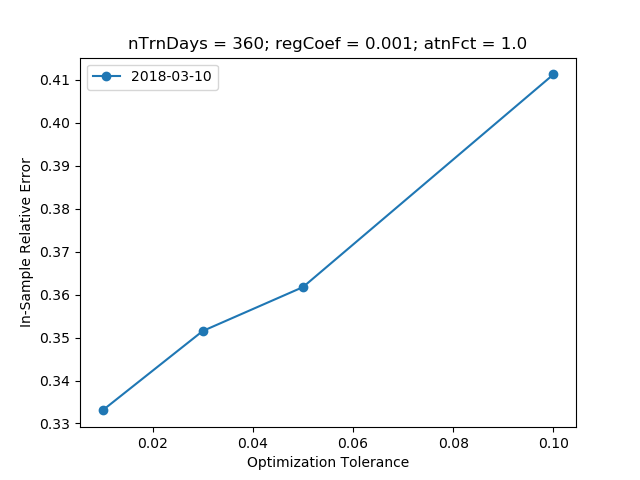
\includegraphics[scale=0.9,bb=0 0 640 480]{figures/tolerance-sensitivity-error.png}
\caption{In-sample relative error vs. optimization tolerance; $T$ =
  360 days, $\eta(t) = 1.0$, $\zeta$ = 1.0e-3.}
\label{fig:tolerance-sensitivity-error}
\end{figure}

\begin{figure}
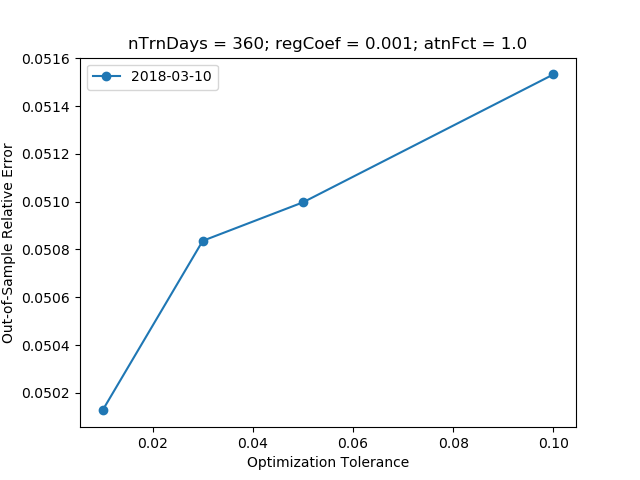
\includegraphics[scale=0.9,bb=0 0 640 480]{figures/tolerance-sensitivity-oos-error.png}
\caption{Out-of-sample relative error vs. optimization tolerance; $T$
  = 360 days, $T^{oos}$ = 3, days$\eta(t)$ = 1.0, $\zeta$ = 1.0e-3.}
\label{fig:tolerance-sensitivity-oos-error}
\end{figure}

\begin{figure}
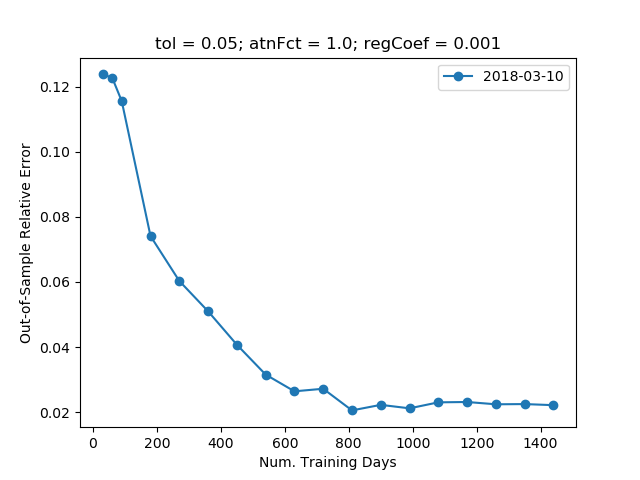
\includegraphics[scale=0.9,bb=0 0 640 480]{figures/nTrnDays-sensitivity-oos-error.png}
\caption{Out-of-sample relative error vs. number of days used for
  training; $T^{oos}$ = 3, $\eta(t)$ = 1.0, $\zeta$ = 1.0e-3,
  tolerance = 0.05.}
\label{fig:nTrnDays-sensitivity-oos-error}
\end{figure}

\begin{figure}
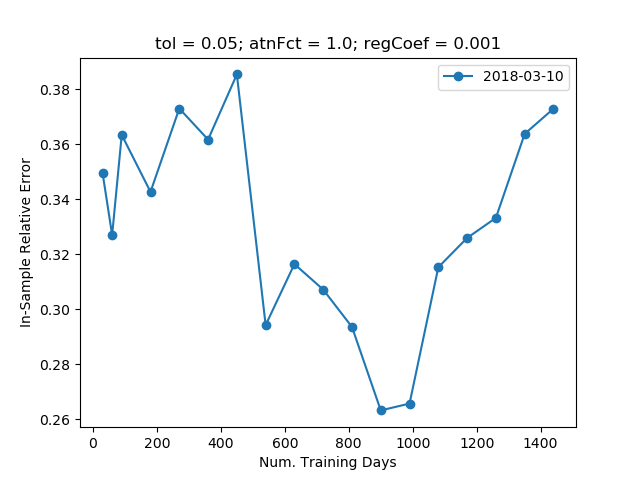
\includegraphics[scale=0.9,bb=0 0 640 480]{figures/nTrnDays-sensitivity-error.png}
\caption{In-sample relative error vs. number of days used for
  training; $\eta(t) = 1.0$, $\zeta$ = 1.0e-3, tolerance = 0.05.}
\label{fig:nTrnDays-sensitivity-error}
\end{figure}

\begin{figure}
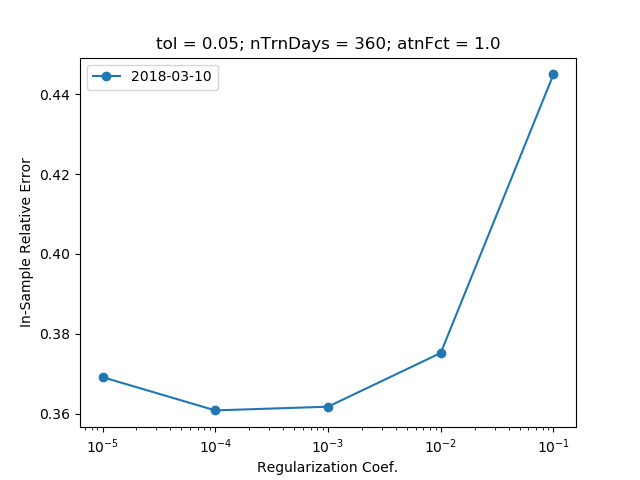
\includegraphics[scale=0.9,bb=0 0 640 480]{figures/regCoef-sensitivity-error.png}
\caption{In-sample relative error vs. regularization coefficient; $T$
  = 360 days, $\eta(t)$ = 1.0, tolerance = 0.05.}
\label{fig:regCoef-sensitivity-error}
\end{figure}

\begin{figure}
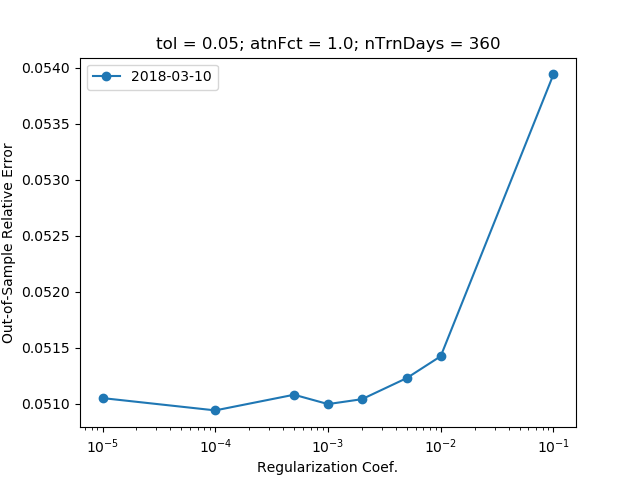
\includegraphics[scale=0.9,bb=0 0 640 480]{figures/regCoef-sensitivity-oos-error.png}
\caption{Out-of-sample relative error vs. regularization coefficient;
  $T$ = 360 days, $T^{oos}$ = 3, $\eta(t)$ = 1.0, tolerance = 0.05.}
\label{fig:regCoef-sensitivity-oos-error}
\end{figure}

\begin{figure}
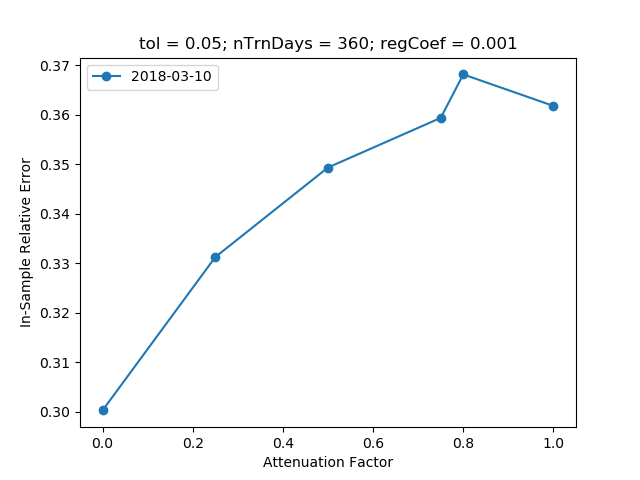
\includegraphics[scale=0.9,bb=0 0 640 480]{figures/atnFct-sensitivity-error.png}
\caption{In-sample relative error vs. attenuation parameter; $T$ = 360
  days, $\zeta$ = 1.0e-3, tolerance = 0.05.}
\label{fig:atnFct-sensitivity-error}
\end{figure}

\begin{figure}
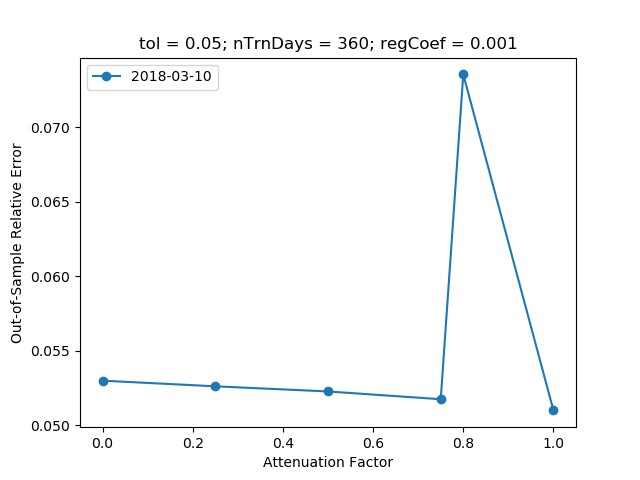
\includegraphics[scale=0.9,bb=0 0 640 480]{figures/atnFct-sensitivity-oos-error.png}
\caption{Out-of-sample relative error vs. attenuation parameter; $T$ =
  360 days, $T^{oos}$ = 3, $\zeta$ = 1.0e-3, tolerance = 0.05.}
\label{fig:atnFct-sensitivity-oos-error}
\end{figure}

\begin{figure}
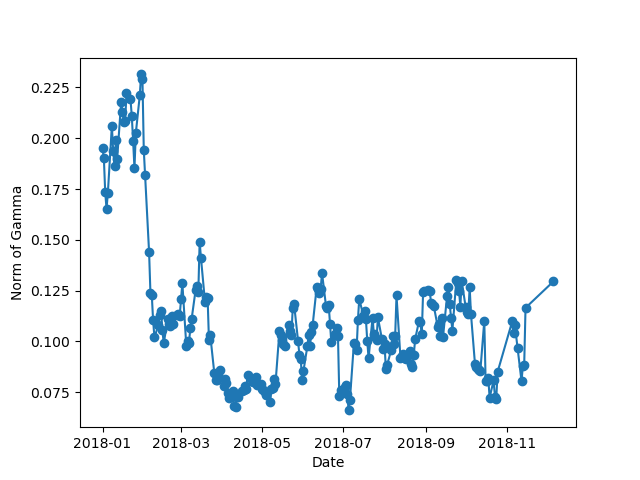
\includegraphics[scale=0.9,bb=0 0 640 480]{figures/Gamma_time_2018.png}
\caption{Norm of Gamma vs. snapdate Each point on the plot comes from
  a model with a constant Christoffel symbol; for all models we have
  $T$ = 360 days, $\zeta$ = 1.0e-3, $\eta_{0}$ = 1.0, tolerance =
  0.05.}
\label{fig:gamma-time}
\end{figure}

\begin{figure}
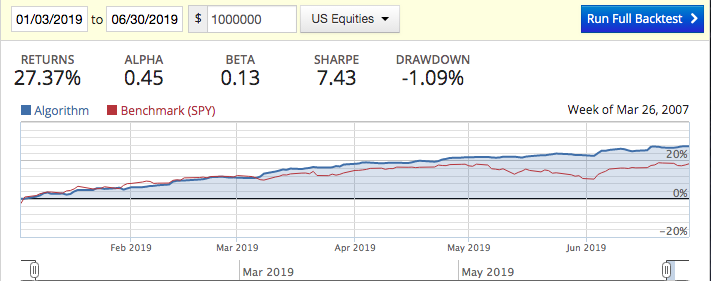
\includegraphics[scale=0.5,bb=0 0 640 480]{figures/2019_half_mfd_macd.png}
\caption{Comparison of proposed algorithm (blue) to SPY (red); first
  half of 2019.}
\label{fig:backtest-2019-half}
\end{figure}

\begin{figure}
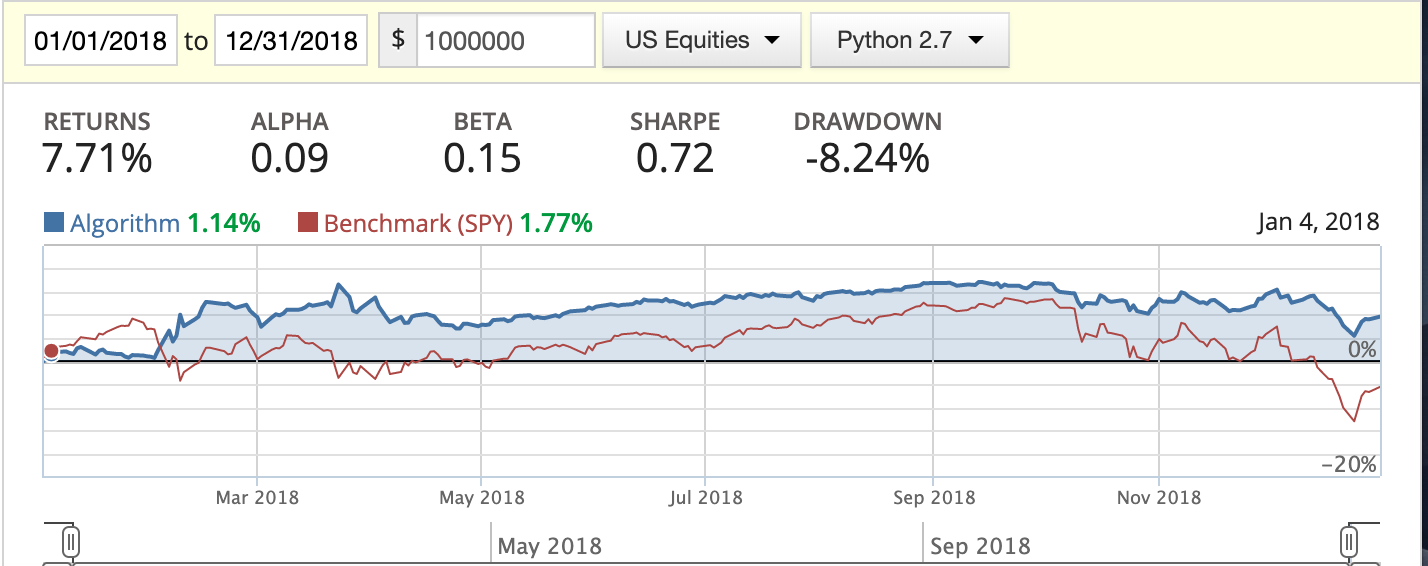
\includegraphics[scale=0.5,bb=0 0 640 480]{figures/mad_mfd_macd_2018.png}
\caption{Comparison of proposed algorithm (blue) to SPY (red); 2018.}
\label{fig:backtest-2018}
\end{figure}

\begin{figure}
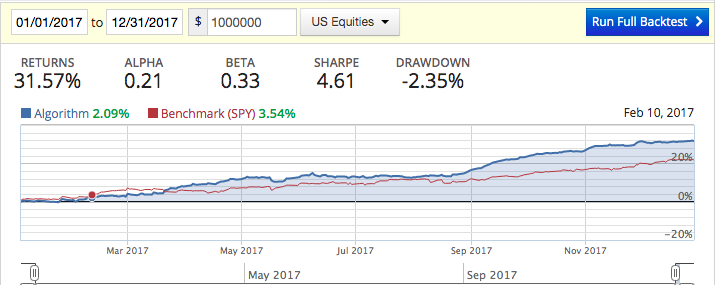
\includegraphics[scale=0.5,bb=0 0 640 480]{figures/mad_mfd_macd_2017.png}
\caption{Comparison of proposed algorithm to SPY; 2017.}
\label{fig:backtest-2017}
\end{figure}

\begin{figure}
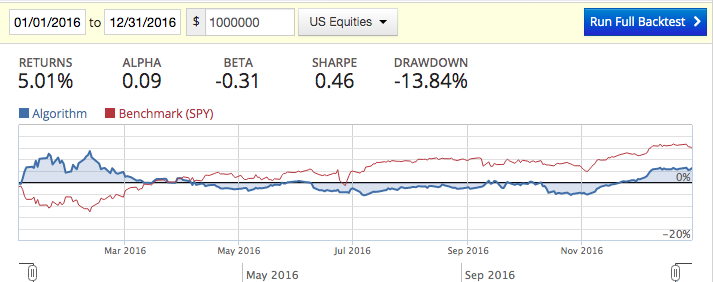
\includegraphics[scale=0.5,bb=0 0 640 480]{figures/mad_mfd_macd_2016.png}
\caption{Comparison of proposed algorithm to SPY; 2016.}
\label{fig:backtest-2016}
\end{figure}

\begin{figure}
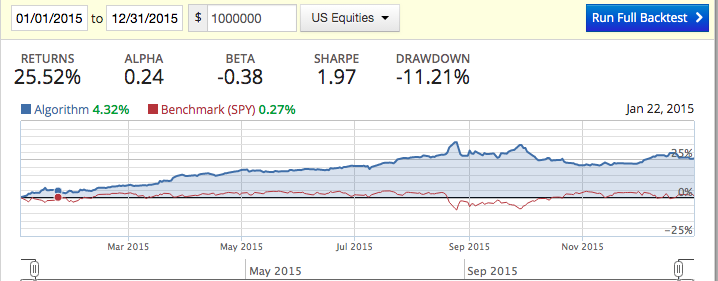
\includegraphics[scale=0.5,bb=0 0 640 480]{figures/mad_mfd_macd_2015.png}
\caption{Comparison of proposed algorithm to SPY; 2015.}
\label{fig:backtest-2015}
\end{figure}

\begin{figure}
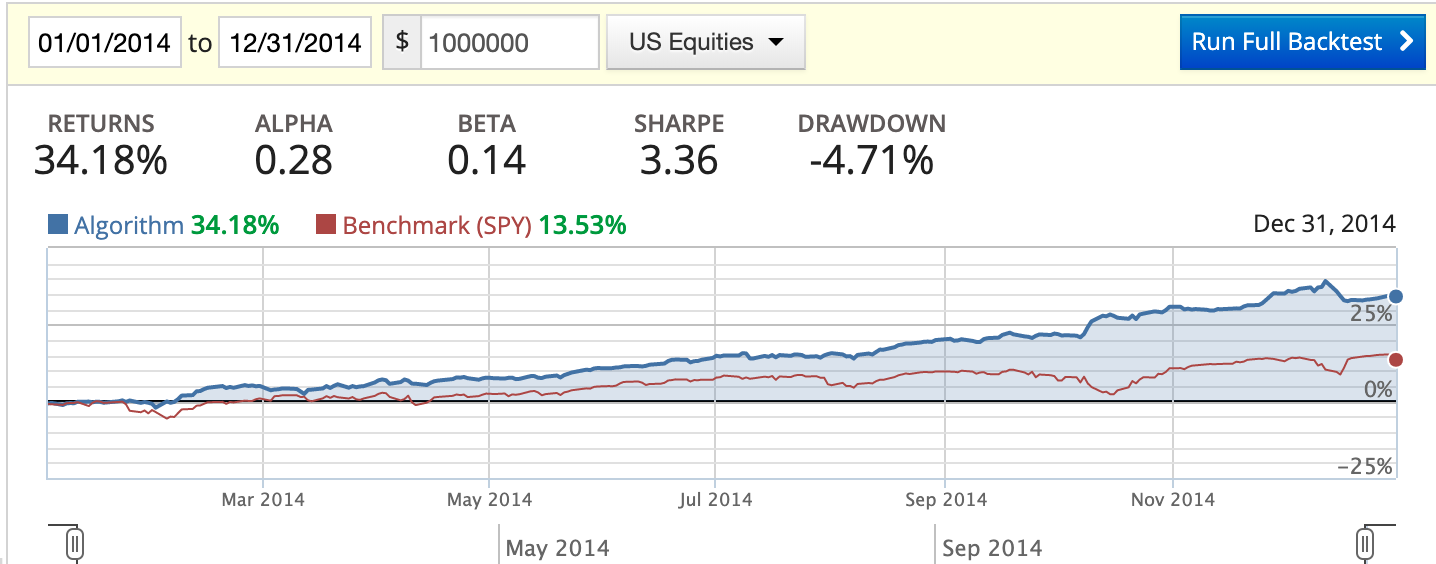
\includegraphics[scale=0.5,bb=0 0 640 480]{figures/mad_mfd_macd_2014.png}
\caption{Comparison of proposed algorithm to SPY; 2014.}
\label{fig:backtest-2014}
\end{figure}

\begin{figure}
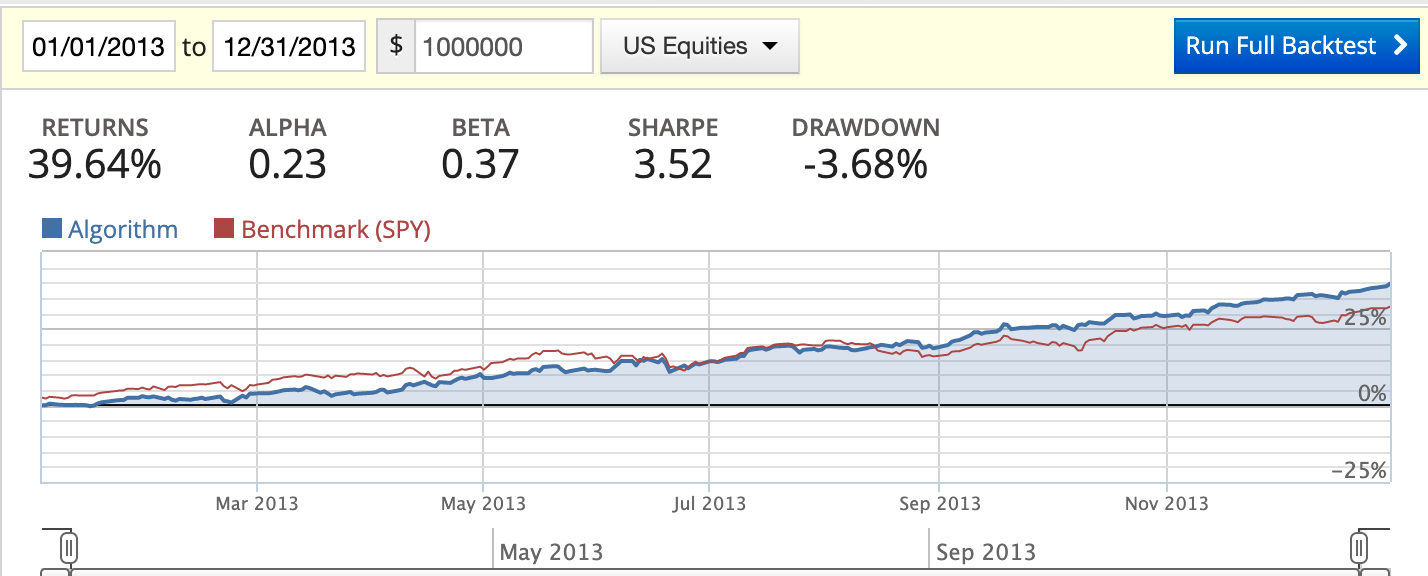
\includegraphics[scale=0.5,bb=0 0 640 480]{figures/mad_mfd_macd_2013.png}
\caption{Comparison of proposed algorithm to SPY; 2013.}
\label{fig:backtest-2013}
\end{figure}

\begin{figure}
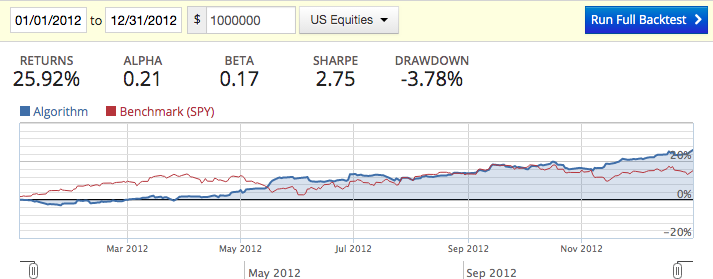
\includegraphics[scale=0.5,bb=0 0 640 480]{figures/mad_mfd_macd_2012.png}
\caption{Comparison of proposed algorithm to SPY; 2012.}
\label{fig:backtest-2012}
\end{figure}

\begin{figure}
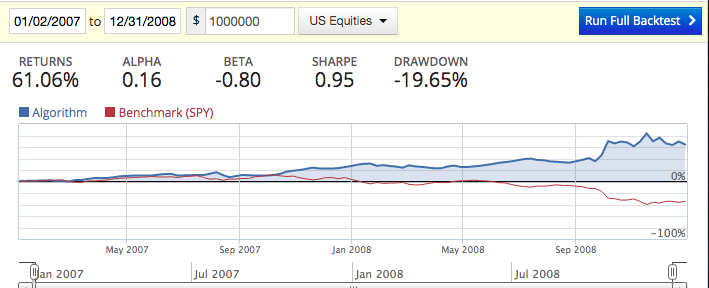
\includegraphics[scale=0.5,bb=0 0 640 480]{figures/crash_period_mfd_macd.png}
\caption{Comparison of proposed algorithm to SPY; 2007-2008.}
\label{fig:backtest-2007-2008}
\end{figure}

\begin{figure}
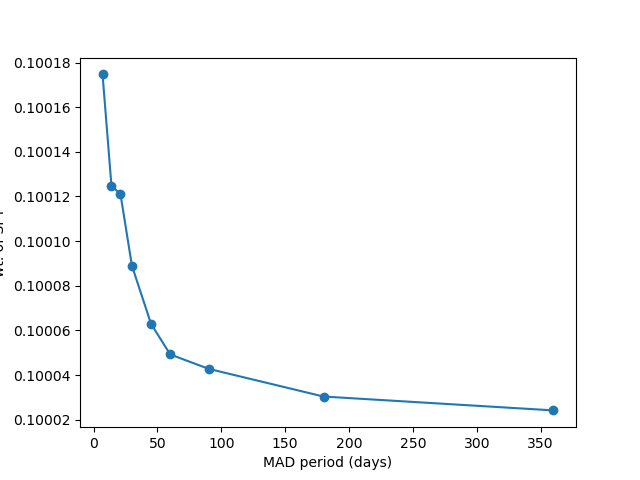
\includegraphics[scale=0.9,bb=0 0 640 480]{figures/mad-sensitivity-period-SPY.png}
\caption{The weight of SPY vs. period used for calculation of MAD.}
\label{fig:mad-period-sensitivity}
\end{figure}

\clearpage

\bibliography{references}
\bibliographystyle{plain}

\end{document}

